\chapter{بررسی نتایج و ارزیابی مدل‌های ارائه شده}


\section{آزمایش‌های انجام‌شده بر روی پیکره «تاج»}
پس از استخراج یک مجموعه داده در حوزه اخبار جعلی، به ارزیابی مدل‌های ارائه شده می‌پردازیم. همانطور که در بخش \ref{section.pretrained_models} عنوان شد، چندین مدل از پیش آموزش‌ دیده برای زبان‌ فارسی موجود است. در این بخش ما با استفاده از دسته‌بند‌های ذکرشده، پیچشی و پرسپترون، یک مقایسه میان این مدل‌ها انجام می‌دهیم تا بهترین مدل‌ را برای تشخیص اخبار جعلی فارسی انتخاب کنیم. به منظور اثبات کارایی مدل‌های ارائه‌شده، ما از دادگان دیگر فارسی و انگلیسی نیز برای ارزیابی استفاده می‌کنیم.

\subsection{تنظیمات آزمایش‌ها}
مدل‌های برت چندزبانه و ایکس.ال.ام-روبرتا دارای نسخه‌های متفاوتی است. در این پژوهش، ما از نسخه‌ پایه هر دو مدل استفاده کردیم. مدل برت چند‌زبانه پایه دارای ۱۷۹ میلیون پارامتر قابل آموزش، ۱۲ لایه انتقال‌دهنده و لایه میانی با اندازه ۷۶۸ است. مدل ایکس.ال.ام-روبرتا پایه نیز دارای ۲۷۰ میلیون پارامتر، ۱۲ لایه انتقال‌دهنده و لایه‌میانی با اندازه ۷۶۸ است. مدل‌های دیگر مانند پارس‌برت و آلبرتا-فارسی همگی بر پایه مدل برت است.

معماری دسته‌بند پیچشی شامل ۳ لایه پیچشی موازی شامل ۳۰ فیلتر‌ با ابعاد متفاوت ۳ و ۴ و ۵ است که ویژگی‌های سطح بالاتر را از ماتریس خروجی مدل ازپیش‌ آموزش‌دیده که شامل یک بردار مجزا برای هر کلمه ورودی است، استخراج می‌کند. لایه آخر این دسته‌بند نیز یک پرسپترون ساده است که با استفاده از تابع بیشینه‌هموار\LTRfootnote{Softmax}، برچسب هر خبر را مشخص می‌کند. به‌منظور جلوگیری از مشکل بیش‌برازش\LTRfootnote{Overfit} در مدل نیز از پارامتر‌های تنظیم‌کننده در فیلتر‌ها استفاده شده ‌است.

شبکه عصبی پیشرو پرسپترون نیز شامل یک لایه پرسپترون با تابع فعال‌ساز بیشینه‌هموار است که با استفاده از بردار خروجی مدل از پیش آموزش‌ دیده به محاسبه احتمال تعلق یک خبر به هر کدام از دسته‌ها می‌پردازد.

در تمامی مدل‌ها نیز یک لایه بیرون‌انداز\LTRfootnote{Dropout Layer} قبل از لایه‌ نهایی قرار گرفته‌ است. همچنین در آموزش مدل‌ها نرخ یادگیری\LTRfootnote{Learning Rate} در آموزش برابر با $5e-5$، تعداد دوره‌‌ها\LTRfootnote{Epoch} برابر با ۴ و مقدار اندازه دسته\LTRfootnote{Batch Size} ۶۴  است.

\subsection{نتایج}
جدول \ref{table.text_result_cnn} نتایج ارزیابی مدل‌های ارائه‌شده با استفاده از مدل‌های از پیش آموزش‌ دیده متفاوت و با استفاده از شبکه عصبی پیچشی را نمایش می‌دهد. طبق نتایج به‌دست‌آمده می‌توان نتیجه گرفت که مدل پارس‌برت نسبت‌ به بقیه‌ مدل‌ها توانسته‌ است متن‌های ورودی را دقیق‌تر بازنمایی کند و ما با استفاده از این مدل می‌توانیم اخبار جعلی را با دقت بالاتری نسبت‌به سایر مدل‌ها تشخیص دهیم.

\begin{table}
	\caption{نتایج تشخیص اخبار جعلی فارسی با استفاده از بازنمایی‌های مختلف و دسته‌بندی با شبکه عصبی پیچشی}
	\label{table.text_result_cnn}
	\begin{center}
		\begin{tabular}{|c|c|c|c|c|}
			\hline
مدل & فراخوانی & صحت & معیار اف & دقت \\
			\hline
			\hline
برت چندزبانه & $88.55$ & $84$ & $86.21$ & $87.33$\\
			\hline
آلبرت-فارسی & $87.02$ & $92$ & $89.44$ & $89.75$ \\
			\hline
پارس برت & $89.13$ & $93.71$ & $91.36$ & $91,64$ \\
			\hline
ایکس.ال.ام-روبرتا & $87.84$ & $90.85$ & $89.32$ & $89.75$ \\
			\hline
		\end{tabular}
	\end{center}
\end{table}

در گام بعدی، در مدل پارس برت علاوه‌بر دسته‌بندی با شبکه پیچشی، دسته‌بندی با شبکه پیشرو پرسپترون تک‌لایه نیز مورد بررسی قرار گرفت که نتایج آن در جدول \ref{table.text_result_slp} گزارش شده‌ است. همان‌طور که نتایج این جدول نشان می‌دهد شبکه پرسپترون تک‌لایه به نتایج نزدیکی در مقایسه با شبکه پیچشی رسیده‌ است و با تفاوت اندک به دقت و معیار اف بالاتری دست یافته ‌است. بر اساس این نتایج، بازنمایی پارس‌برت در سطح واژه به‌ همراه شبکه پیچشی و بازنمایی پارس‌برت در سطح متن به همراه شبکه پیشرو پرسپترون در گام‌های بعدی این پروژه مورد استفاده قرار خواهد گرفت.

\begin{table}
	\caption{نتایج تشخیص اخبار جعلی فارسی با استفاده از بازنمایی پارس‌برت و مقایسه دسته‌بندها}
	\label{table.text_result_slp}
	\begin{center}
		\begin{tabular}{|c|c|c|c|c|c|}
			\hline
مدل & دسته‌بند & فراخوانی & صحت & معیار اف & دقت \\
			\hline
			\hline
پارس برت & شبکه عصبی پیچشی  & $89.13$ & $93.71$ & $91.36$ & $91.64$ \\
			\hline
پارس برت & شبکه پیشرو پرسپترون تک‌لایه & $92.44$ & $90.85$ & $91.64$ & $92.18$ \\
			\hline
		\end{tabular}
	\end{center}
\end{table}

\section{آزمایش‌های انجام‌شده بر روی سایر پیکره‌های فارسی}
همانطور که ذکر شد، از آنجا که دادگان تهیه‌شده در این پروژه برای اولین بار در زمینه تشخیص خبر جعلی مورد استفاده قرار می‌گیرد، نتایج پایه دیگری بر روی این دادگان به‌منظور مقایسه وجود ندارد. بر همین اساس، به‌‌منظور ارزیابی مدل‌های ارائه‌شده برای زبان فارسی و مقایسه نتایج این پروژه با کارهای قبلی انجام‌شده در زبان فارسی، ما از دو مجموعه داده موجود برای تشخیص شایعات در شبکه‌های اجتماعی توییتر و تلگرام استفاده کردیم. مدل‌های پایه‌ای که برای مقایسه استفاده شده ‌است در ادامه مرور می‌شوند:
\begin{itemize}
\item
\cite{zamani2017rumor}
یک روش مبتنی‌ بر مدل «بهینه‌سازی کمینه متوالی»\LTRfootnote{Sequetional Minimal Optimization (SMO)} که یک روش آموزش ماشین بردار پشتیبان است برای تشخیص شایعات فارسی در شبکه اجتماعی تلگرام ارائه داده‌اند. ما در این بخش از آزمایش‌ها مدل ارائه‌شده در این پروژه را با مدل ارائه‌شده توسط \cite{zamani2017rumor} مقایسه نموده‌ایم. در این مقایسه از دادگانی که توسط \cite{zamani2017rumor} ارائه گردیده است استفاده کرده‌ایم. شایان ذکر است در مقاله ارائه‌شده توسط ایشان، علاوه بر اطلاعات متنی، از ویژگی‌های مرتبط با گراف کاربران توییتر نیز استفاده کرده‌اند، اما به‌دلیل عدم دسترسی به این اطلاعات، مقایسه ما تنها با بخشی از مدل‌های ارائه‌شده توسط \cite{zamani2017rumor}  که برروی دادگان متنی پیاده شده است  انجام پذیرفته ‌است.

\item
\citet{jahanbakhsh2020model}
با ارائه مدل مبتنی‌ بر ماشین بردار پشتیبان به دسته‌بندی شایعات در شبکه اجتماعی توییتر پرداختند. ما در بخش دیگری از آزمایش‌ها از دادگان توییتر ارائه‌شده توسط \citet{jahanbakhsh2020model} استفاده کردیم و مدل خود را با نتایج آن‌ها مقایسه نمودیم.

جدول \ref{table.comparison} نتایج حاصل از مدل‌های پیاده‌شده در این پژوهش را بر روی دو مجموعه داده حاصل از تلگرام و توییتر نشان می‌دهد. در این آزمایش‌ها از مدل زبانی پارس‌برت استفاده شده‌است.


\begin{table}
	\caption{ارزیابی و مقایسه مدل‌های ارائه‌شده با مدل‌های پیشین برروی دادگان فارسی شبکه‌های اجتماعی}
	\label{table.comparison}
	\begin{center}
		\begin{tabular}{|c|c|c|c|c|c|}
			\hline
			مدل & دادگان & فراخوانی & صحت & معیار اف & دقت \\
			\hline
			\hline
			\citep{zamani2017rumor} & 
			\multirow{4}{*}{توییتر} &$71.44$&$81.24$& $76.02$ & $74.26$ \\
			
			\cline{1-1}
			\cline{3-6}
			\citep{jahanbakhsh2020model} &
			 & $76.3$ & $76.3$ & $76.3$ & - \\
			\cline{1-1}
			\cline{3-6}
			پارس‌برت - پیچشی & & $95.71$ & $97.10$ & $96.40$ & $96.12$ \\
			\cline{1-1}
			\cline{3-6}
			پارس‌برت - پرسپترون & & $94.20$ & $94.20$ & $94.20$ & $93.79$ \\
			\hline
			\citep{jahanbakhsh2020model} &
			\multirow{3}{*}{تلگرام}& $82.8$ & $82.9$ & $82.8$ & - \\
			\cline{1-1}
			\cline{3-6}
			پارس‌برت - پیچشی & & $93.49$ & $95.04$ & $94.26$ & $92.51$ \\
			\cline{1-1}
			\cline{3-6}
			پارس‌برت - پرسپترون & & $92.06$ & $95.86$ & $93.92$ & $91.97$ \\
			\hline
		\end{tabular}
	\end{center}
\end{table}
\end{itemize}
	
	همانطور که از نتایج مشخص است، مدل‌های ارائه شده با استفاده از بازنمائی‌ مبتنی بر مفهوم به صورت چشمگیری معیار‌های ارزیابی را بهبود دادند. همچنین، دسته‌بند پیچشی درمقایسه با مدل شبکه پرسپترون پیشرو عملکرد بهتری داشته است چراکه در این حالت مدل پیچشی ویژگی‌های سطح بالاتری را براساس هم‌نشینی واژگان ایجاد می‌کند. با توجه به آزمایش‌های انجام شده برروی دادگان توییتر، مدل پارس‌برت-پیچشی ۲۰ درصد معیار اف را در مقایسه با مدل‌های ارائه شده توسط \cite{zamani2017rumor} و \cite{jahanbakhsh2020model} بهبود‌ داده‌است. علاوه بر این، این مدل توانست برروی دادگان تلگرام نیز معیار اف را در مقایسه با نتایج بدست‌آمده توسط \cite{jahanbakhsh2020model} 
	۱۱ درصد ارتقا دهد.
	
\section{آزمایش‌های انجام‌شده برروی پیکره‌های زبان انگلیسی}
همان‌طورکه پیش‌تر مطرح شد، برای تشخیص خبر جعلی فارسی ابتدا شاکله‌ی یک مدل را براساس داده انگلیسی می‌سازیم و سپس با تغییر داده به فارسی، مدل را با داده فارسی آموزش داده و آن را بهینه می‌کنیم. ازاین‌رو، در ادامه، مدل آموزش‌ داده‌ شده با داده انگلیسی توضیح داده می‌شود. برای استفاده از دادگان لیار از ویژگی متن خبر و ۵ ویژگی مرتبط با تاریخچه اعتبار هر عنوان خبر استفاده می‌گردد. 
تاریخچه اعتبار هر گوینده شامل تعداد اخبار «به‌سختی درست»، «جعلی»، «نیمه درست»، «عمدتاً درست» و «دروغ» که از این گوینده تا کنون منتشر شده‌است می‌باشد.
علاوه بر آنها، تمامی ۶ برچسب که پیش‌تر معرفی شده بود به ۲ دسته «جعلی» و «اصیل» نگاشت می‌شود و برچسب زده می‌شوند؛
به این صورت که برچسب‌های «درست»، «نیمه درست» و «عمدتاً درست» به دسته اصیل و برچسب‌های «جعلی»،  «دروغ» و «به‌سختی درست» به دسته جعلی نگاشت می‌شوند.  در \tablename~\ref{table.LiarResults2} نتایج حاصل از ارزیابی این دادگان در حالت ۲ برچسب «جعلی» و «اصیل» با استفاده از دو مدل برت و شبکه عصبی پیچشی نمایش داده شده‌است. در این جدول، مدل حاصل از شبکه پیچشی که از ورد۲وک\LTRfootnote{Word2vec}\citep{mikolov2013distributed} برای تعبیه‌ واژه‌ها استفاده شده‌است به‌عنوان مدل پایه مورد استفاده و مقایسه قرار گرفته‌است.  همچنین در \figurename~\ref{LIAR-CM} ماتریس درهم‌ریختگی دو مدل «برت + پرسپترون ساده» و «برت +‌ پیچشی» و مدل پایه نمایش داده شده‌است.

\begin{table}[!h]
	\caption{نتایج آزمایش مدل‌های ارائه‌شده بر روی دادگان لیار (۲ برچسب)}
	\label{table.LiarResults2}
	\begin{center}
		\begin{tabular}{|M{4cm}|c|c|c|c|c|}
			\hline
			مدل & بازنمایی & فراخوانی & صحت & دقت & معیار اف \\
			\hline
			\hline
			شبکه عصبی پیچشی‌ & 
			ورد۲وک & 
			$58.58$ &
			$48.14$ & 
			$54.34$ & 
			$52.84$ \\
			\hline
			شبکه عصبی پیچشی‌ & 
			برت & 
			$62.92$ &
			$67.05$ & 
			$70.30$ & 
			$64.91$ \\
			\hline
			پرسپترون ساده & 
			برت & 
			$64.37$ &
			$66.04$ & 
			$69.98$ & 
			$65.19$ \\
			\hline
		\end{tabular}
	\end{center}
\end{table}

\begin{table}[!h]
	\caption{ مقایسه مدل‌های ارائه شده با مدل‌های پایه براساس دادگان لیار (۶ برچسب)}
	\label{table.LiarResults6}
	\begin{center}
		\begin{tabular}{|M{6cm}|c|c|c|}
			\hline
			مدل & بازنمایی & دقت تست & دقت اعتبارسنجی \\
			\hline
			\hline
			ال.اس.تی.ام مکانیزم توجه  &
			\multirow{2}{*}{ورد۲وک} &
			\multirow{2}{*}{$38.5$} &
			\multirow{2}{*}{$37.8$} \\
			\citep{long2017fake} &  &  &  \\
			\hline
			
			شبکه کپسولی &
			\multirow{2}{*}{ورد۲وک}&
			\multirow{2}{*}{$39.5$} &
			\multirow{2}{*}{$40.9$}\\
			\citep{goldani2020detecting} & &  & \\
			\hline\hline
			
			\multirow{2}{*}{شبکه عصبی پیچشی}& 
			ورد۲وک & 
			$39.3$ &
			$39.8$ \\
			\cline{2-4}
			& 
			برت & 
			$44.1$ &
			$45.5$ \\
			\hline
			پرسپترون ساده & 
			برت & 
			\textbf{$45.1$} &
			\textbf{$48.4$} \\
			\hline
		\end{tabular}
	\end{center}
\end{table}

\begin{figure}[!h]
	\centering
	\begin{tabular}{ccc}
		\begin{subfigure}{0.33\textwidth}
			\centering
			\caption{ورد۲وک + پیچشی}
			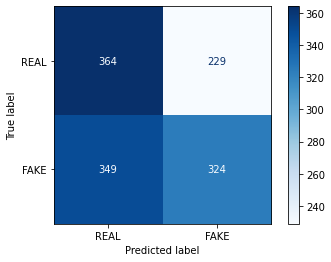
\includegraphics[width=1 \textwidth]{cnn-liar2-cm}
		\end{subfigure}
		& 
		\begin{subfigure}{0.33\textwidth}
			\centering
			\caption{برت + پیچشی}
			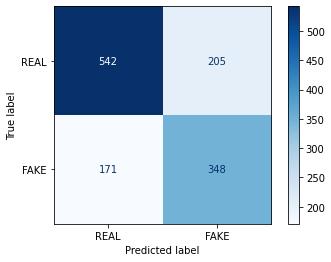
\includegraphics[width=1 \textwidth]{bert-cnn-liar2-cm}
		\end{subfigure}
		&
		\begin{subfigure}{0.33\textwidth}
			\centering
			\caption{برت + پرسپترون ساده}
			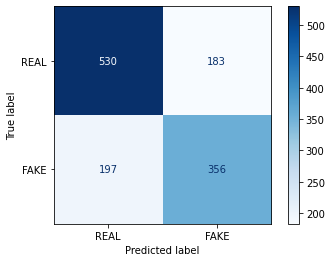
\includegraphics[width=1 \textwidth]{bert-slp-liar2-cm}
		\end{subfigure}
	\end{tabular}
	\caption{ ماتریس درهم‌ریختگی نتایج آزمایش‌های دادگان لیار}
	\label{LIAR-CM}
\end{figure}

همان‌طورکه در \tablename~\ref{table.LiarResults2}  مشاهده می‌شود، مدل پرسپترون ساده با استفاده از بازنمایی تولیدشده توسط مدل برت نتیجه بهتری را برای این مجموعه دادگان داشته‌ و با دقت بالاتری اخبار جعلی را تشخیص داده‌است.  در این مدل، میزان خطای مثبت کاذب که نشانگر تعداد اخبار جعلی است که توسط سیستم به خطا اصیل تشخیص داده شده‌است کمتر از سایر مدل پیشنهادی ما می‌باشد.

برای مقایسه مدل پیشنهادی با سایر مدل‌های مطرح و به‌ روز، نتایج آزمایش مدل‌های این طرح با مدل‌هایی که پیش‌تر برای دسته‌بندی اخبار دادگان لیار با ۶ برچسب ارائه شده‌ است در\tablename~ \ref{table.error_liar_fn} نمایش داده شده‌ است.  باتوجه‌به نتایج، مدل پرسپترون ساده با استفاده از بازنمایی برت نسبت‌به دیگر مدل‌ها با دقت بالاتری اخبار لیار را دسته‌بندی کرده ‌است.

برای بررسی خطا در مدل‌های ارائه شده، در ادامه دو نمونه از اخباری که به اشتباه در آزمایش مدل «برت + پرسپترون» دسته‌بندی شده‌است، مورد بررسی قرار می‌گیرد. ابتدا سابقه گوینده‌ی هر دو خبر در  \tablename~\ref{table.error_history_liar_fn}  نمایش داده شده‌ است.  در ادامه  \tablename~\ref{table.error_liar_fn}   آمار واژگان نمونه  (۱)   را نمایش می‌دهد که یک خبر جعلی است و به اشتباه در دسته اخبار اصیل قرار گرفته‌است. همچنین  \tablename~\ref{table.error_liar_fp}   آمار واژگان نمونه  (۲)   را نشان می‌دهد که یک خبر اصیل است و به اشتباه در دسته جعلی قرار گرفته‌است. 



(۱)\\
\begin{flushleft}\lr{Citizens Property Insurance has over \$500 billion worth of risk, with less than \$10 billion worth of surplus.}\end{flushleft}

(۲)\\
\begin{flushleft}\lr{Says the unemployment rate for college graduates is 4.4 percent and over 10 percent for noncollege-educated.}\end{flushleft}

\begin{table}[!h]
	\caption{آمار تاریخچه گوینده دو نمونه خبر  1  و  2 }
	\label{table.error_history_liar_fn}
	\begin{center}
		\begin{tabular}{|c|c|c|c|c|c|}
			\hline
			نمونه & به‌سختی درست & جعلی & دروغ & عمدتاً درست & نیمه درست \\
			\hline
			\hline
			نمونه  1  & 28 & 23 & 7 & 34 & 38 \\ \hline
			نمونه  2  & 12 & 16 & 5 & 7 & 13 \\ \hline
		\end{tabular}
	\end{center}
\end{table}


\begin{table}[!h]
	\caption{آمار واژگان یک نمونه  1  (خبر جعلی دسته‌بندی‌شده در دسته خبر اصیل)}
	\label{table.error_liar_fn}
	\begin{center}
		\begin{tabular}{|c|c|c|}
			\hline
			واژه هدف & تعداد واژه در اخبار جعلی & تعداد واژه در اخبار اصیل \\
			\hline
			\hline
			\lr{citizen} & 35 & 40 \\ \hline
			\lr{properti} & 37 & 43 \\ \hline
			\lr{insur} & 98 & 121 \\ \hline
			\lr{billion} & 193 & 229 \\ \hline
			\lr{worth} & 3 & 25 \\ \hline‌
			\lr{risk} & 13 & 15 \\ \hline
			\lr{less} & 53 & 197 \\ \hline
			\lr{surplu} & 13 & 19 \\ \hline
		\end{tabular}
	\end{center}
\end{table}


\begin{table}[!h]
	\caption{آمار واژگان نمونه  2  (خبر اصیل دسته‌بندی‌شده در دسته خبر جعلی) }
	\label{table.error_liar_fp}
	\begin{center}
		\begin{tabular}{|c|c|c|}
			\hline
			واژه هدف & تعداد واژه در اخبار جعلی & تعداد واژه در اخبار اصیل \\
			\hline
			\hline
			\lr{say} & 1222 & 1281 \\ \hline
			\lr{unemploy} & 65 & 122 \\ \hline
			\lr{rate} & 121 & 284 \\ \hline
			\lr{colleg} & 35 & 91 \\ \hline
			\lr{graduat} & 13 & 51 \\ \hline‌
			\lr{percent} & 351 & 836 \\ \hline
			\lr{noncollegeeduc} & 0 & 1 \\ \hline
		\end{tabular}
	\end{center}
\end{table}


باتوجه‌به آمار واژگان و همچنین سابقه گوینده می‌توان نتیجه گرفت که هم سابقه فرد و هم واژگان به‌کاررفته در این دو نمونه خبر ماهیتی متفاوت از برچسب صحیح  را دارد و شباهت اطلاعات موجود در واژگان و سابقه گوینده به دسته دیگر سبب خطای مدل پیشنهادشده ما شده‌است.


در آزمایش با دادگان ای.آس.اُ.تی. نیز از ویژگی متن خبر به تنهایی استفاده شده‌است که نتایج مقایسه آن با مدل های پیشین \citet{ahmed2017detection} و مدل شبکه کپسولی \citep{goldani2020detecting} در \tablename~\ref{table.ISOTResults} گزارش شده‌است. در این دادگان نیز مدل شبکه پیچشی با استفاده از ورد۲وک به‌عنوان مدل پایه به‌کار رفته‌است. طبق نتایج گزارش‌شده در این جدول، دو مدل پرسپترون ساده و شبکه عصبی پیچشی که از بازنمایی مدل برت استفاده کردند دقت بالاتری را نسبت‌به مدل‌های پیشین ثبت کردند. 

در \figurename~\ref{ISOT-CM} نیز ماتریس درهم‌ریختگی حاصل از ارزیابی مدل‌های ارائه شده برروی دادگان آی.اس.اُ.تی نمایش داده شده‌است. همان‌طورکه در نتایج مشاهده می‌شود دقت هر دو مدل مبتنی‌بر برت به \%۱۰۰ رسیده‌است و هیچ خطای مثبت کاذب و منفی کاذب در نتایج وجود ندارد.



\begin{table}[!h]
	\caption{ مقایسه مدل‌های ارائه‌شده با مدل‌های پیشین برروی دادگان ای.آس.اُ.تی. }
	\label{table.ISOTResults}
	\begin{center}
		\begin{tabular}{|r|c|c|}
			\hline
			مدل & بازنمایی & دقت \\
			\hline
			\hline
			بردار ماشین پشتیبان &\multirow{7}{*}{ ورد۲وک} & 86 \\
			بردار ماشین پشتیبان خطی &  & 92 \\
			کا نزدیک‌ترین همسایه&  & 83 \\
			درخت تصمیم &  & 89 \\
			گرادیان کاهشی تصادفی &  & 89 \\
			رگرسیون خطی &  & 89 \\
			شبکه کپسولی &  & $99.8$ \\
			\hline 
			\hline 
			\multirow{2}{*}{شبکه عصبی پیچشی} & ورد۲وک & $98.08$ \\
			\cline{2-3}
			& برت & \textbf{100} \\
			\hline
			پرسپترون ساده & برت & \textbf{100} \\
			\hline
		\end{tabular}
	\end{center}
\end{table}

\begin{figure}[!h]
	\centering
	\begin{tabular}{ccc}
		\begin{subfigure}{0.33\textwidth}
			\centering
			\caption{ورد۲وک + پیچشی}
			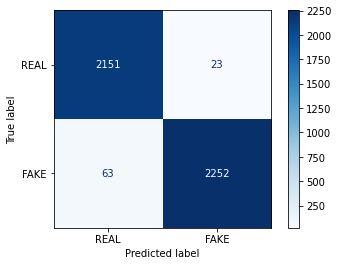
\includegraphics[width=1 \textwidth]{cnn-isot-cm}
		\end{subfigure}
		& 
		\begin{subfigure}{0.33\textwidth}
			\centering
			\caption{برت + پیچشی}
			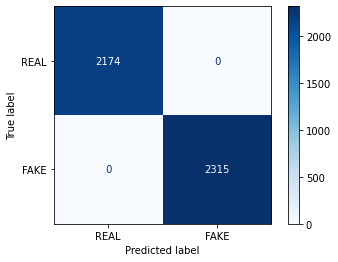
\includegraphics[width=1 \textwidth]{bert-cnn-isot-cm}
		\end{subfigure}
		&
		\begin{subfigure}{0.33\textwidth}
			\centering
			\caption{برت + پرسپترون ساده}
			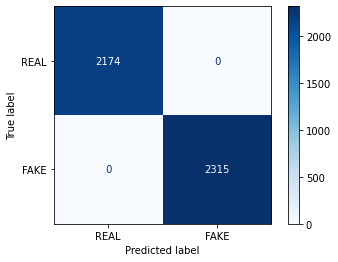
\includegraphics[width=1 \textwidth]{bert-slp-isot-cm}
		\end{subfigure}
	\end{tabular}
	\caption{ماتریس درهم‌ریختگی نتایج آزمایش‌های دادگان آی.اس.اُ.تی.}
	\label{ISOT-CM}
\end{figure}



همان‌طورکه از نتایج ارائه‌شده بر روی دادگان لیار و آی.اس.اُ.تی مشخص است، هر دو مدل «برت +‌ پرسپترون ساده» و «برت + پیچشی» نتایج قابل قبولی نسبت‌به روش‌های پیشین ارائه داده‌است. استفاده از لایه‌های پیچشی پس‌از بازنمایی ارائه شده توسط مدل برت به‌منظور به‌دست‌آوردن بازنمایی سطح بالاتر باتوجه‌به هم‌نشینی واژه‌ها در جمله بوده‌است؛ اما طبق نتایج به‌دست‌آمده توسط مدل پرسپترون ساده، بازنمایی‌های حاصل از مدل برت به میزان قابل قبولی دارای ویژگی‌های مناسبی برای نمایندگی واژه‌ها و جملات است. علاوه‌بر این، از مقایسه مدل «برت +‌ پیچشی» و مدل «ورد۲وک + پیچشی» که تنها از بازنمایی حاصل از همنشینی واژگان استفاده می‌کند، می‌توان نتیجه گرفت که قدرت مدل‌های ارائه‌شده در این بخش از پروژه حاصل از توانایی زیاد مدل برت برای بازنمایی جملات و کلمات است.
